\section{确定项目的前景与范围}

\subsection{引言}

\subsubsection{为什么要确定项目的前景和范围}
在看待现实世界时:世界是复杂的,从不同的角度观察(目的与条件),会看到不同的内容(抽象与映射)。所以会有两个问题:
\begin{itemize}
    \item 如何保证项目涉众以符合项目需要的角度描述现实世界?
    \item 描述哪些事物和事件才会尽可能的符合项目的需要?
\end{itemize}

因此需要
\begin{itemize}
    \item 定义项目前景:所有的涉众都从共同认同的项目前景出发,理解和描述问题域及需求
    \item 定义项目范围:范围内的事物和事件是描述的目标
\end{itemize}

\subsubsection{确定项目前景和范围的关键}
确定项目前景和范围的关键是定义业务需求和能够满足需求的高层解决方案,包括:
\vspace{-0.8em}
	\begin{multicols}{3}
        \begin{itemize}
            \item 业务目标、目的
            \item 高层业务功能
            \item 每个高层业务功能所关联的高层数据
            \item 每个功能相关的项目涉众
            \item ……
        \end{itemize}
	\end{multicols}
\vspace{-1em}
如果存在不同业务需求之间的冲突,那么在确定项目前景和范围阶段必须予以解决

\subsubsection{问题概述}
确定项目的前景与范围,就是确定项目的问题、目标、特性
\begin{itemize}
    \item (业务需求)问题:组织的战略目标、利益分配、政策规划、业务流程等高层问题
    \item 目标:问题的反面,用户的期望
    \item 系统特性(解决问题的方向):选定的、针对目标的解决方案所需要具备的功能特征,通常内聚于一个目标与任务,反映系统与外界一次有价值的完整互动过程(用户)
\end{itemize}

针对项目的复杂程度,针对“范围”可以采用的分析手段由浅到深依次为问题分析、目标分析、业务过程分析
\begin{itemize}
    \item 问题与目标明确$\rightarrow$问题分析$\rightarrow$用例图/上下文图
    \item 目标之间存在较为复杂的关系$\rightarrow$目标分析$\rightarrow$目标模型与目标实现
    \item 目标、特性之间存在紧密的联系$\rightarrow$业务过程分析$\rightarrow$UML活动图
    \item 分析过程越复杂,分析结果的形式化程度越高,变更的成本也越大
\end{itemize}

此外,还需要分析非功能需求,定义系统边界,生成前景与范围文档

\subsection{问题分析}

\subsubsection{获取问题}
问题分析的前提是获取问题,这可以通过收集背景资料或与涉众沟通来实现。

连锁商店获取问题示例:
\vspace{-0.25em}
{\kaishu \begin{compactitem}
    \item P1:手工作业销售迟缓,效率不高。
    \item P2:商店的商品品种太多,无法准确掌握库存。
    \item P3:成本不够低,导致竞争力不强,盈利水平不够。
    \item P4:顾客不够多,销售额不高,盈利水平不够。
\end{compactitem}}

\subsubsection{问题解决方案描述}
\vspace{-0.5em}
\begin{center}
    \begin{longtable}{|Wc{2cm}|Wc{1.5cm}|m{11cm}|}
        \hline
        \multicolumn{2}{|c|}{\textbf{要素}}                          & \multicolumn{1}{c|}{\textbf{内容}}                                                \\ \hline
        \multicolumn{2}{|c|}{ID}                                   & \multicolumn{1}{c|}{P2}                                                          \\ \hline
        \multicolumn{1}{|c|}{\multirow{3}{*}{解决方案1}} & 方案描述        & 准确的库存管理,记录入库和出库,提供实时的库存分析数据,可以及时地发现可能的积压、缺货、报废现象。           \\ \cline{2-3} 
        \multicolumn{1}{|c|}{}                       & 业务优势        & 及时发现积压、缺货与报废,可以尽早处置。                                        \\ \cline{2-3} 
        \multicolumn{1}{|c|}{}                       & 代价          & 对积压、缺货的预测可能不准确,会因此而产生代价。                                    \\ \hline
        \multicolumn{1}{|c|}{\multirow{3}{*}{解决方案2}} & 方案描述        & 制定促销策略,处置可能的积压和报废商品。                                        \\ \cline{2-3} 
        \multicolumn{1}{|c|}{}                       & 业务优势        & 通过促销,可以减少积压和报废商品带来的损失。                                      \\ \cline{2-3} 
        \multicolumn{1}{|c|}{}                       & 代价          & 促销本身会产生代价。                                                  \\ \hline
        \multicolumn{1}{|c|}{\multirow{3}{*}{解决方案3}} & 方案描述        & 根据过去的销售情况预测未来的销售数据,并据此调整商品购买时机和数量。                          \\ \cline{2-3} 
        \multicolumn{1}{|c|}{}                       & 业务优势        & 可以做到成本最小化。                                                  \\ \cline{2-3} 
        \multicolumn{1}{|c|}{}                       & 代价          & 如果预测不准确,产生较多的缺货现象会降低顾客满意度。                                  \\ \hline
        \multicolumn{1}{|c|}{\multirow{3}{*}{解决方案4}} & 方案描述        & 对积压、报废和缺货现象比较频繁的商品进行调整。将总是积压和报废的商品调整出销售目录,为总是缺货的商品引入新的同类商品。 \\ \cline{2-3} 
        \multicolumn{1}{|c|}{}                       & 业务优势        & 可以比较长远地解决积压、缺货、报废现象。                                        \\ \cline{2-3} 
        \multicolumn{1}{|c|}{}                       & 代价 & 无     \\\hline
    \end{longtable}
\end{center}
\vspace{-3.7em}

\subsubsection{面向对象边界描述:用例图}
\vspace{-1em}
\begin{figure}[H]
	\centering
	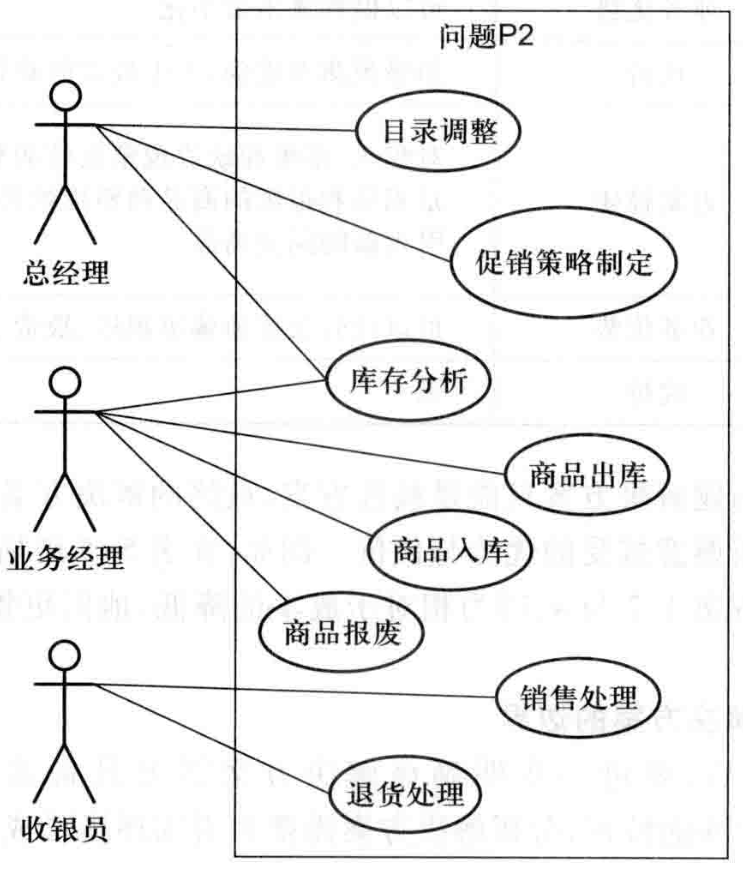
\includegraphics[width=0.32\textwidth]{img/问题P2的用例图.png}
\end{figure}
\vspace{-1em}


\subsection{目标分析}

\subsubsection{“目标”概念——面向目标的需求工程方法}
面向目标的需求工程方法是一种正式定义“目标”概念,并以此为基础开展需求工程活动的方法。也就是说,面向目标需求工程方法中的“目标” 概念是被明确定义的,有相应的方法和技术负责它的解释和使用。

面向目标的需求工程方法是指向整个需求工程的,对当今需求工程方法和技术的影响比较普遍,但是它的核心作用表现在前期需求阶段—一项目前景与范围定义活动。

\subsubsection{目标模型}

\paragraph{目标}~{} \par
日标是系统被开发的目的
\begin{itemize}
    \item 它有着明确的定义方式 
    \item 每个日标都拥有一些特征属性,常见的有类型、名称、说明、优先级、可行性和效用等
\end{itemize}

\begin{figure}[H]
	\centering
	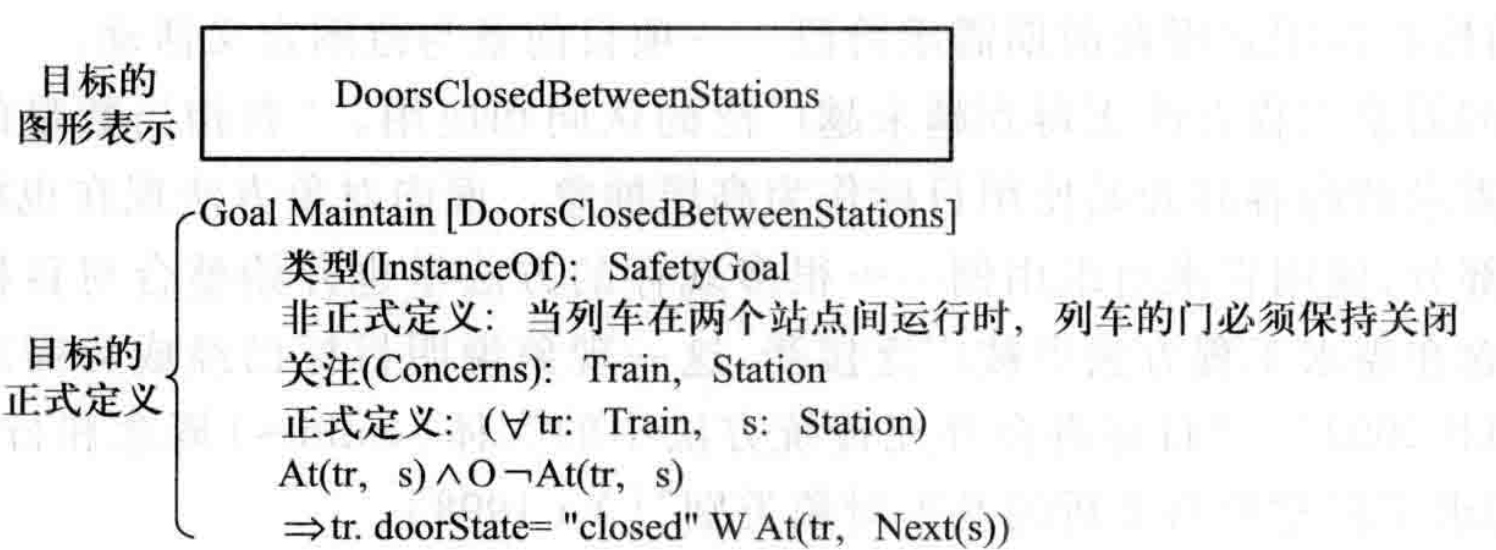
\includegraphics[width=0.7\textwidth]{img/KAOS对目标的描述.png}
    \caption*{KAOS对目标的描述}
\end{figure}
\vspace{-1em}

时序逻辑常用操作符
\begin{table}[H]
    \centering
    \begin{tabular}{|c|c|c|}
    \hline
    操作符 & 用法    & 含义                 \\ \hline
    $\bigcirc$   & $\bigcirc$Q    & 在下一个状态中Q必须为真       \\ \hline
    {\Large $\bullet$}   & {\Large $\bullet$}Q    & 在前一个状态中Q必须为真       \\ \hline
    $\lozenge$   & $\lozenge$Q    & Q终将在未来的某个时间点上为真    \\ \hline
    $\blacklozenge$   & $\blacklozenge$Q    & 过去的某个时间上Q曾经为真      \\ \hline
    $\square$   & $\square$Q    & 在所有后续路径中,Q必须始终为真   \\ \hline
    $\blacksquare$   & $\blacksquare$Q    & 在过去的路径中,Q必须始终为真    \\ \hline
    U   & P\;U\;Q & P必须一直为真直到将来的某一点Q为假 \\ \hline
    W   & P\;W\;Q & P必须一直为真直到将来的某一点Q为真 \\ \hline
    \end{tabular}
\end{table}

目标可以被分成不同的类型
\begin{itemize}
    \item 最常见的是将其分为功能目标和非功能目标
    \begin{itemize}
        \item 功能目标是期望系统提供的服务,可以分为满足型目标和信息型目标。
        \item 非功能目标是期望系统满足的质量,常见的是质量目标和约束目标。非功能目标可以依据质量模型的属性细分为安全目标、性能目标和可用性目标等。
    \end{itemize}
    \item 目标又可以被分为软目标和硬目标。
    \begin{itemize}
        \item 软目标是指无法清晰判断是否满足的目标,如关于可维护性的目标。
        \item 硬目标则是那些可以通过一些技术确认其是否满足的目标,如关于性能指标的目标。
    \end{itemize}
\end{itemize}


依据其正式定义的特点,[Dardenne 1993]将目标总结为5种基本模式,并以此为基础进行目标的规格与关系处理[Darimont 1996]
\vspace{-0.5em}
\begin{table}[H]
    \centering
    \begin{tabular}{|c|c|c|}
        \hline
        模式  &	符号描述  &	含义 \\\hline
        实现(Achieve) & $\mathrm{P} \Rightarrow \lozenge \mathrm{Q}$ & 如果将来某一时刻Q为真(被满足),则目标实现 \\\hline
        终止(Cease) & $\mathrm{P} \Rightarrow \lozenge \lnot \mathrm{Q}$ & 如果将来某一时刻Q为假(被终止),则目标实现 \\\hline
        保持(Maintain) & $\mathrm{P} \Rightarrow \square \mathrm{Q}$ & 将来任一时刻Q都为真,则目标实现 \\\hline
        避免(Avoid) & $\mathrm{P} \Rightarrow \square \lnot \mathrm{Q}$ & 将来任一时刻Q都为假,则目标实现 \\\hline
        优化(Optimize) & — & 最大化Maximize(目标功能)或最小化Minimize(目标功能)\\\hline
    \end{tabular}
\end{table}
\vspace{-1em}

\paragraph{关系}~{} \par
除了核心的目标概念之外,目标模型的另一个核心要素是元素之间的关系,又称为链接
\vspace{-0.8em}
	\begin{multicols}{3}
        \begin{itemize}
            \item 精化关系
            \item 阻碍关系
            \item 支持与冲突关系
        \end{itemize}        
	\end{multicols}
\vspace{-1em}

\textbf{目标精化} \par
一个高层次目标G可以精化为低层次目标\{G1, G2, …, G$n$\}
\begin{itemize}
    \item 如果一系列子目标\{G1, G2, …, G$n$\}的完成有助于目标G的完成,那么G与\{G1, G2, …, G$n$\}之间就是AND精化关系。此时任意两子目标G$i$与G$j$之间是互补的。
    
    如果更进一步,子目标\{G1, G2, …, G$n$\}的完成能够直接保证G的完成,\{G1, G2, …, G$n$\}$\vDash $G,那么G与\{G1, G2, …, G$n$\}之间就是完备(Complete)AND 精化关系。
    \item 如果任一子目标Gi都是G的替代方案,那么G与\{G1, G2, …, G$n$\}之间就是OR精化关系。此时,任意两子目标G$i$与G$j$之间是互相替代的。
\end{itemize}

\textbf{目标阻碍} \par
如果子目标O的达成会使得高层目标G失败,O$\vDash \lnot$ G,那么O与G的关系就是阻碍关系。
\begin{figure}[H]
	\centering
	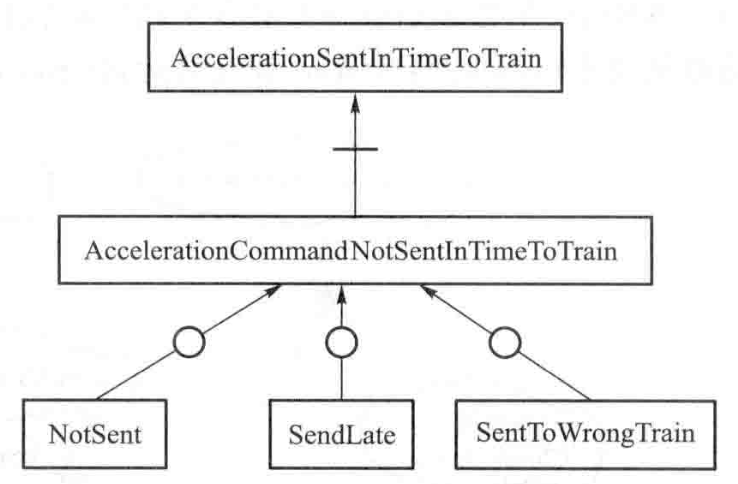
\includegraphics[width=0.45\textwidth]{img/目标模型阻碍关系示意图.png}
    \caption*{目标模型阻碍关系示意图}
\end{figure}
\vspace{-1em}

\textbf{目标之间的支持与冲突关系} \par
支持、冲突关系是对多个目标之间关系的考虑
\begin{itemize}
    \item Support链接表示一个目标对其他目标的支持作用,支持关系可以被处理为OR精化关系
    \item Conflict链接表示一个目标的实现对其他目标的实现有阻碍作用  
\end{itemize}

在二元的支持、冲突关系中,也可以使用如下标识标记关系
\begin{itemize}
    \item ++ (Make):一个目标的成功可以直接保证另一个目标的成功
    \item + (Help):一个目标的成功可以让另一个目标更容易成功
    \item $-$ (Hurt):一个目标的成功会使得另一个目标的成功更加困难
    \item $--$ (Break):一个目标的成功会直接导致另一个目标的失败
\end{itemize}

\begin{figure}[H]
	\centering
	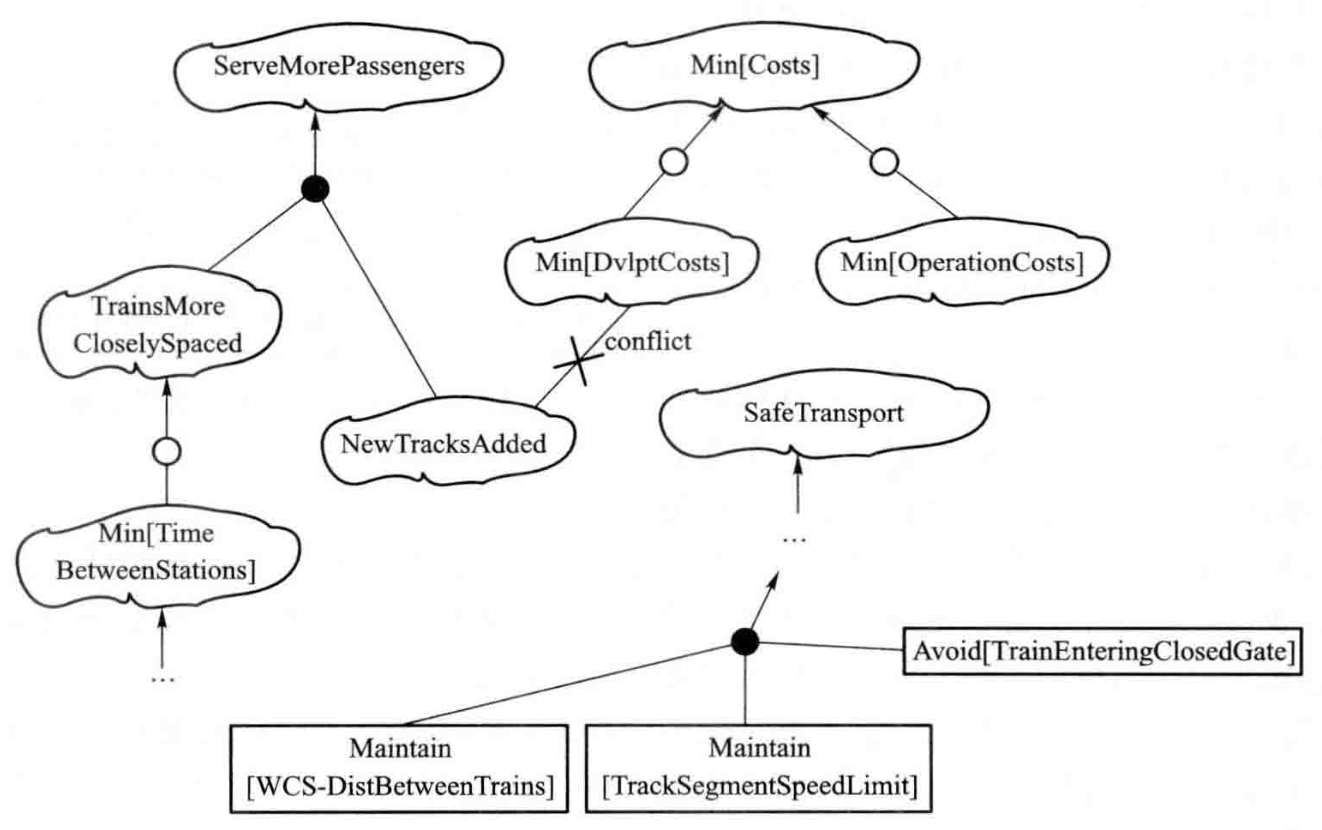
\includegraphics[width=0.7\textwidth]{img/目标模型精化关系示意图.png}
    \caption*{目标模型精化关系示意图}
\end{figure}
\vspace{-1em}

\textbf{目标与其他需求模型元素的链接} \par
目标可以与其他模型元素建立关系,这些模型元素有主体(agent)、场景(scenario)、操作(operation)、任务(task)、资源(resource)和UML元素等。

\begin{figure}[H]
	\setcounter{subfigure}{0}
	\centering
	\vspace{-1em}	
	\subfloat[目标与主体之间的关系示例]{
		\begin{minipage}[t]{0.54\linewidth}
		\centering
		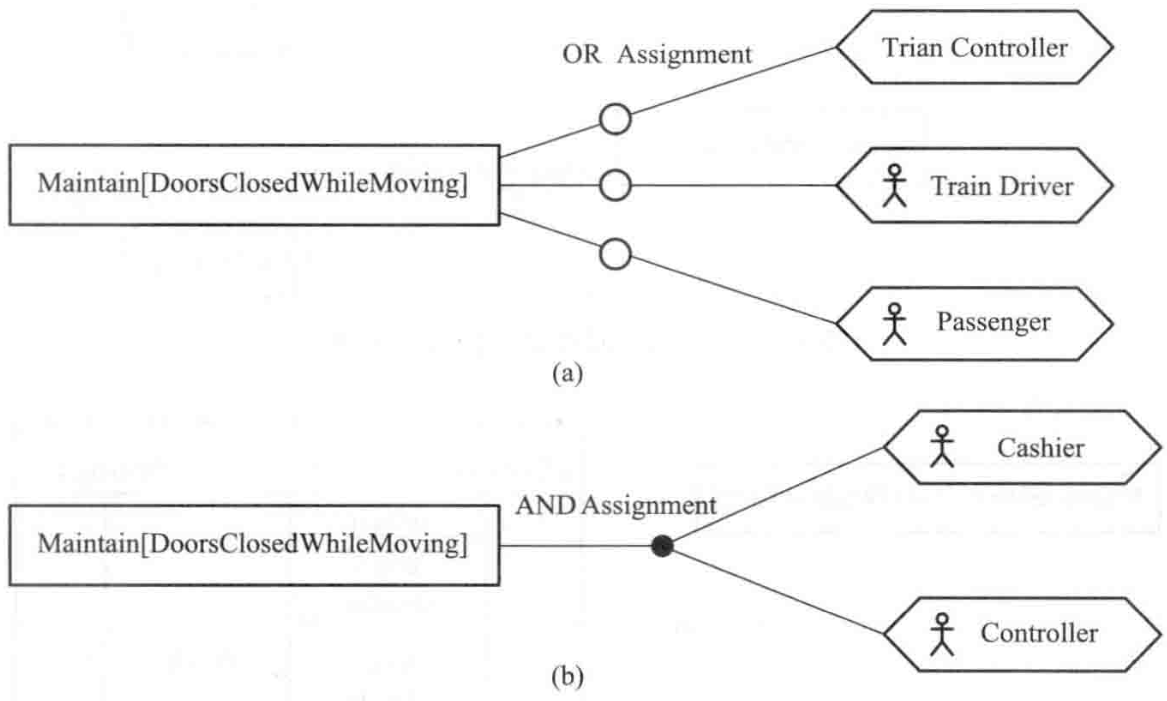
\includegraphics[width=\linewidth]{img/目标与主体之间的关系示例.png}
		\end{minipage}
	}
	\subfloat[目标与操作之间的关系示例]{
		\begin{minipage}[t]{0.43\linewidth}
		\centering
		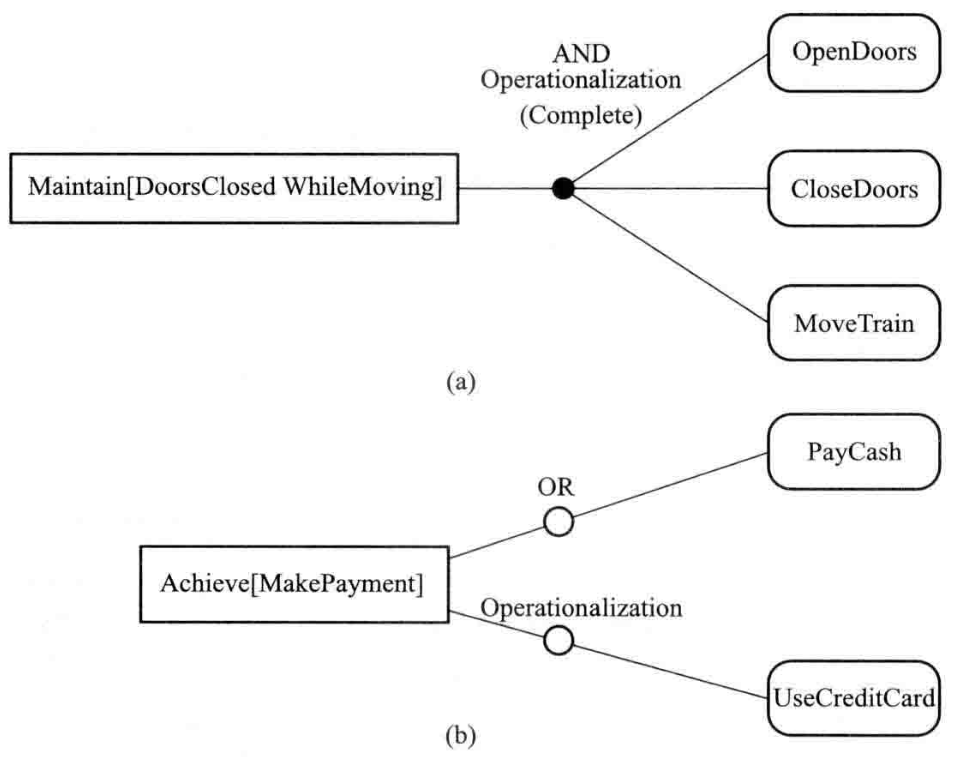
\includegraphics[width=\linewidth]{img/目标与操作之间的关系示例.png}
		\end{minipage}
	}
	\centering
	\vspace{-1em}
\end{figure}

\subsubsection{面向目标的方法}
面向目标方法的处理过程 
\begin{itemize}
    \item 高层目标的获取:现状和背景的分析(画布、评估)
    \item 低层目标的获取 :需求获取与目标分析
    \begin{itemize}
        \item 已有目标的验证和细化 (基于目标分析)
        \item 基于场景的方法等等 (基于目标实现)
    \end{itemize}
    \item 目标分析 :精化与分解
    \begin{itemize}
        \item 建立系统的目标模型 
    \end{itemize}
    \item 目标实现 
    \begin{itemize}
        \item 收集与目标相关的需求信息,讨论可能的候选解决方案,确定最终的系统详细需求和解决方案 
    \end{itemize}
\end{itemize}

\begin{figure}[H]
	\centering
	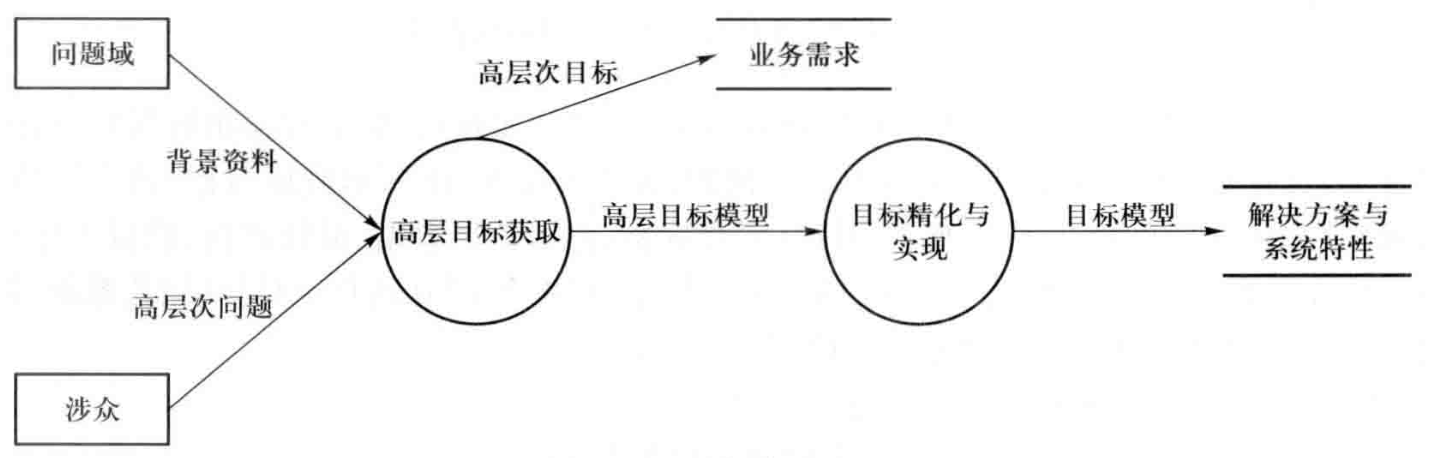
\includegraphics[width=0.85\textwidth]{img/目标分析过程.png}
\end{figure}

\paragraph{高层目标的获取}~{} \par
对于连锁商店销售系统项目,通过分析其问题P1$\sim$P4, 并建立最高层目标BR1$\sim$BR4,这些目标可以被抽取定义为业务需求并将它们组织为目标模型。

\begin{figure}[H]
	\centering
	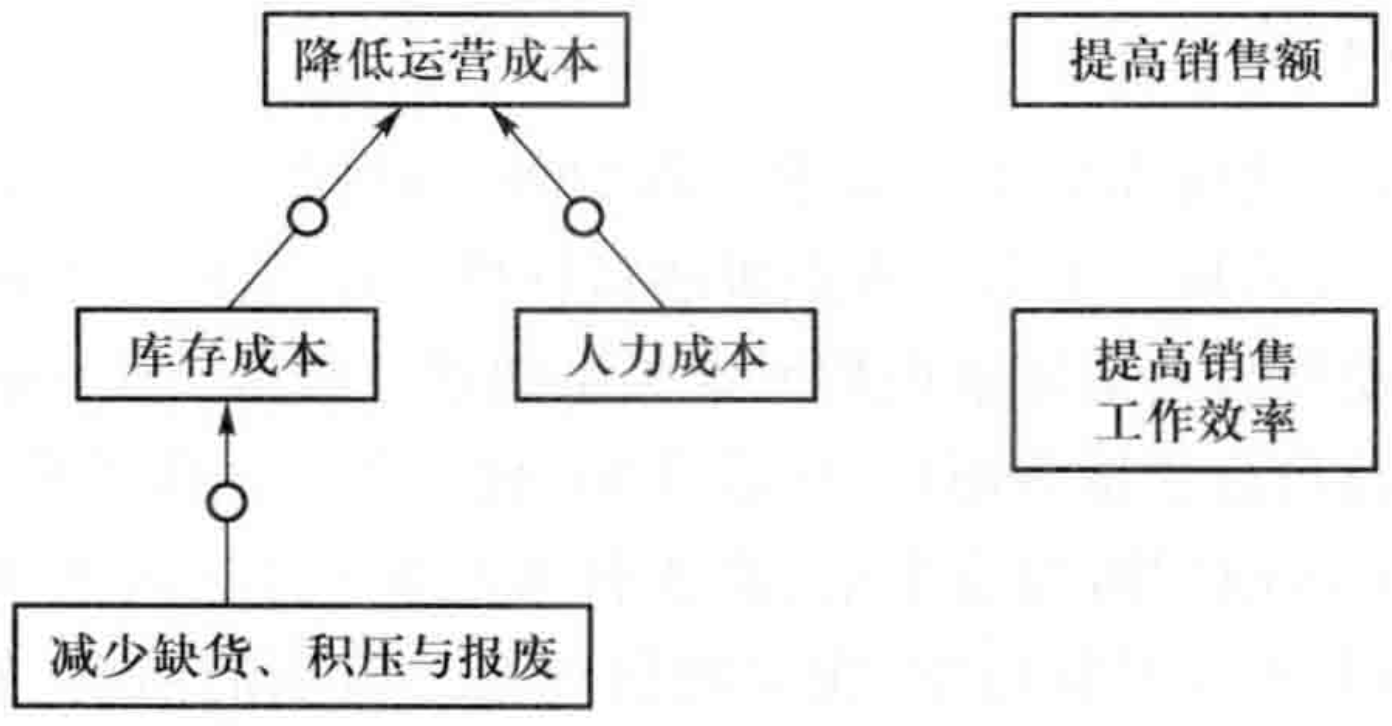
\includegraphics[width=0.48\textwidth]{img/连锁商店销售系统的高层目标模型.png}
    \caption*{连锁商店销售系统的高层目标模型}
\end{figure}
\vspace{-1em}

\paragraph{目标精化}~{} \par

\ding{172} 获取对高层目标的描述

通过收集背景资料,运用面谈、原型等需求获取方法,可以收集对高层目标的描述信息。常见的描述信息包括企业规章、政策,任务描述,业务过程和场景描述。

\ding{173} 从高层目标描述中发现AND精化关系

\begin{itemize}
    \item 同一个目标有不同场景:每个G$i$代表一个典型场景,任意G$i$与G$j$代表不同的场景;
    \item 完成目标有连续过程:每个G$i$代表G完成过程中的一个状态,G$i$、G$i+1$代表两个连续的状态;
    \item 完成目标需要有多个方面紧密配合:G$i$与G$j$紧密联系或互相支持;
    \item 目标有不同质量环境及表现:每个G$i$代表不同质量要求下的G的完成。
\end{itemize}

\ding{174} 从高层目标描述中发现“候选办法”,发现OR精化关系

\ding{175} 考虑阻碍目标(avoid目标)实现的情况

\ding{176} 发现目标冲突关系

\ding{177} 对高层目标问“How”,对低层目标同“Why”,完善层次结构

\vspace{-2em}
\begin{figure}[H]
	\centering
	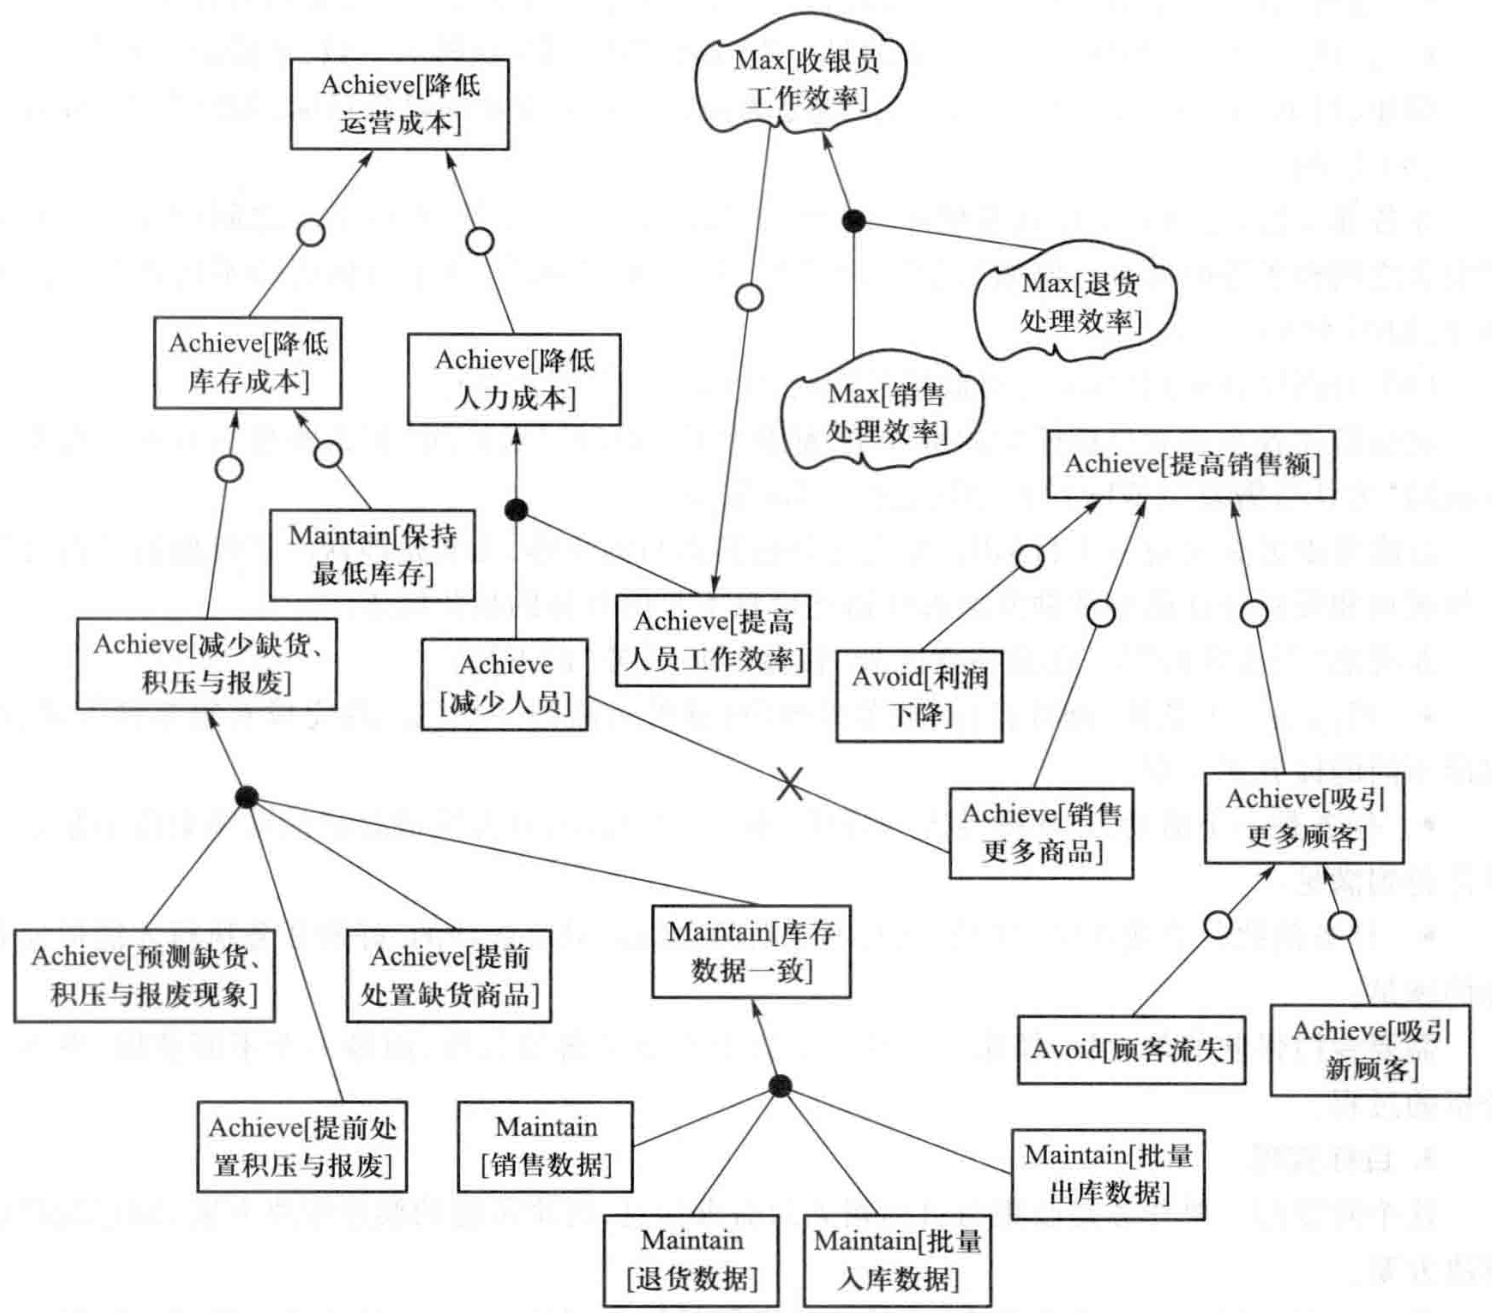
\includegraphics[width=0.88\textwidth]{img/连锁商店销售系统的完整目标模型.png}
    \caption*{\textbf{连锁商店销售系统的完整目标模型}}
\end{figure}
\vspace{-1em}

\paragraph{目标实现}~{} \par
将最底层目标分配给主体(人$+$系统)
\begin{figure}[H]
	\centering
	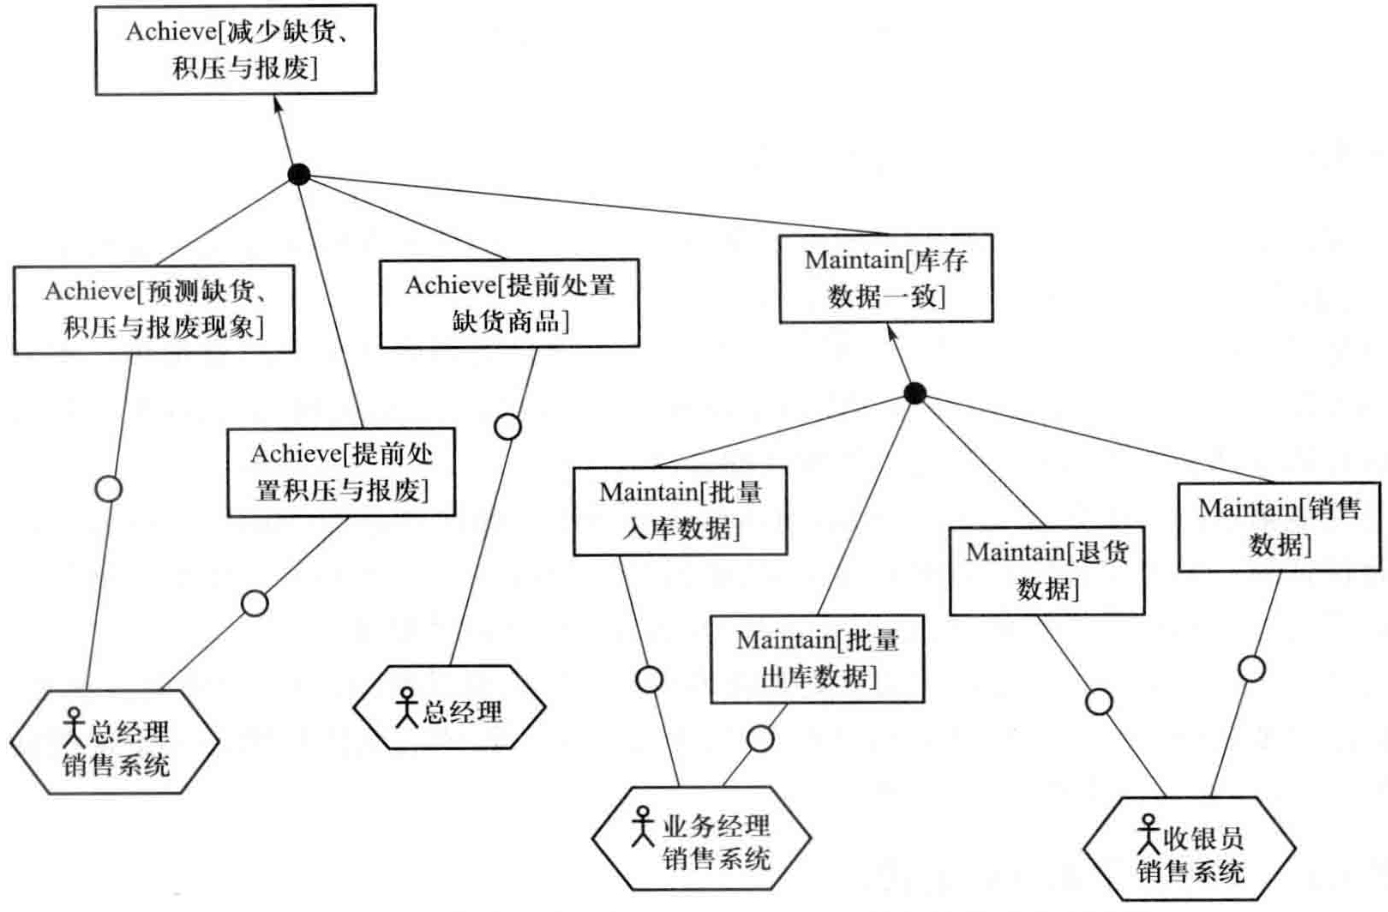
\includegraphics[width=0.75\textwidth]{img/连锁商店销售系统的目标模型片段的主体分配实现示例.png}
    \caption*{连锁商店销售系统的目标模型片段的主体分配实现示例}
\end{figure}
\vspace{-1em}

设计实现最底层目标的操作(任务:细粒度用例/场景)
\begin{figure}[H]
	\centering
	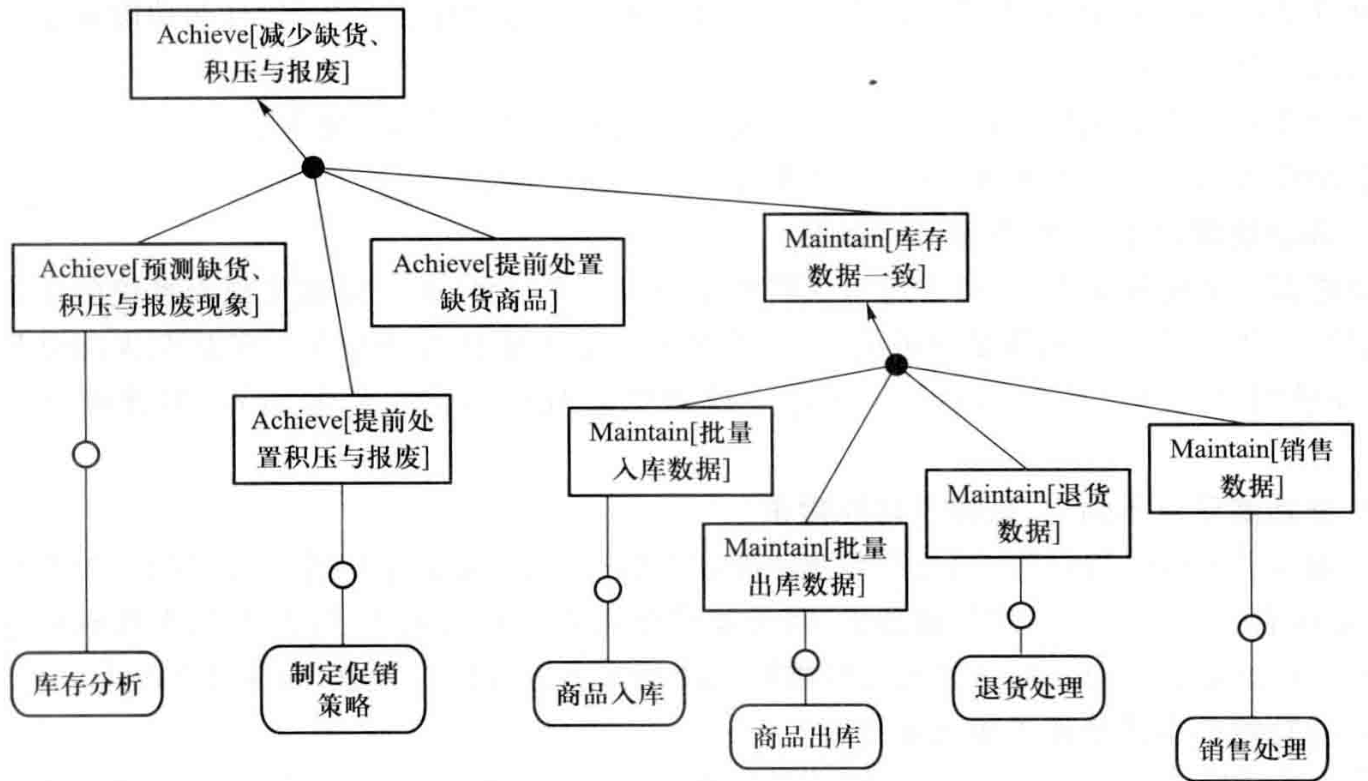
\includegraphics[width=0.85\textwidth]{img/连锁商店销售系统的目标模型片段的操作实现示例.png}
    \caption*{连锁商店销售系统的目标模型片段的操作实现示例}
\end{figure}
\vspace{-1em}